%%%  Ukázkový text a dokumentace stylu pro text závěrečné (bakalářské a
%%%  diplomové) práce na KI PřF UP v Olomouci
%%%  Copyright (C) 2012 Martin Rotter, <rotter.martinos@gmail.com>
%%%  Copyright (C) 2014 Jan Outrata, <jan.outrata@upol.cz>


%%  Pro získání PDF souboru dokumentu je třeba tento zdrojový text v
%%  LaTeXu přeložit (dvakrát) programem pdfLaTeX.

%%  V případě použití programu BibLaTeX pro tvorbu seznamu literatury
%%  je poté ještě třeba spustit program Biber s parametrem jméno
%%  souboru zdrojového textu bez přípony a následně opět (dvakrát)
%%  přeložit zdrojový text programem pdfLaTeX.

%%  Postup získání Postscriptového souboru je popsán v dokumentaci.


%%  Třída dokumentu implementující styl pro závěrečnou práci. Vybrané
%%  nepovinné parametry (ostatní v dokumentaci):

%%  'master' pro sazbu diplomové práce, jinak se sází bakalářská práce

%%  'field=kód' pro Váš studijní obor, kódy pro diplomovou práci 'uvt'
%%  pro Učitelství výpočetní techniky pro střední školy a 'binf' pro
%%  Bioinformatiku, jinak je výchozí Informatika, a pro bakalářskou
%%  práci 'ainfk' pro Aplikovanou informatiku v kombinované formě,
%%  'inf' pro Informatiku, 'infv' pro Informatiku pro vzdělávání a
%%  'binf' pro Bioinfomatiku, jinak je výchozí Aplikovaná informatika
%%  v prezenční formě

%%  'printversion' pro sazbu verze pro tisk (nebarevné logo a odkazy,
%%  odkazy s uvedením adresy za odkazem, ne odkazy do rejstříku),
%%  jinak verze pro prohlížeč

%%  'biblatex' pro zapnutí podpory pro sazbu bibliografie pomocí
%%  BibLaTeXu, jinak je výchozí sazba v prostředí thebibliography

%%  slovak pro slovenský, jinak je výchozí czech pro český

%%  'font=sans' pro bezpatkový font (Iwona Light), jinak výchozí
%%  patkový (Latin Modern)

\documentclass[
%  master,
  field=inf,
%  printversion,
  biblatex,
%  language=english,
%  font=sans,
  glossaries,
  index
]{kidiplom}

%% Informace pro úvodní strany. V jazyku práce (pokud není v komentáři
%% uvedeno česky) a anglicky. Uveďte všechny, u kterých není v
%% komentáři uvedeno, že jsou volitelné. Při neuvedení se použijí
%% výchozí texty. Text pro jiný než nastavený jazyk práce (nepovinným
%% parametrem language makra \documentclass, výchozí český) se zadává
%% použitím makra s uvedením jazyka jako nepovinného parametru.

%% Název práce, česky a anglicky. Měl by se vysázet na jeden řádek.
\title{Grafický editor s výstupem do HTML}
\title[english]{Graphic editor with export to HTML}

%% Volitelný podnázev práce, česky a anglicky. Měl by se vysázet na
%% jeden řádek. Výchozí je prázdný.
\subtitle{}
\subtitle[english]{}

%% Jméno autora práce. Makro nemá nepovinný parametr pro uvedení
%% jazyka.
\author{Zdeněk Mazurák}

%% Jméno vedoucího práce (včetně titulů). Makro nemá nepovinný
%% parametr pro uvedení jazyka.
\supervisor{RNDr. Arnošt Večerka}

%% Volitelný rok odevzdání práce. Výchozí je aktuální (kalendářní)
%% rok. Makro nemá nepovinný parametr pro uvedení jazyka.
%\yearofsubmit{\the\year}

%% Anotace práce, včetně anglické (obvykle překlad z jazyka
%% práce). Jeden odstavec!
\annotation{Cílem této bakalářské práce je vytvoření grafického editoru pro Windows.
Aplikace umožní uživateli kreslit a editovat grafické tvary a text. Všem objektům bude možno nastavit výplň či okraj barvou či gradientem. Editor bude umožňovat export do formátu HTML.}

\annotation[english]{The aim of this bachelor's thesis is to create the graphic editor for Windows. The application will allow the user to draw and edit graphical shapes and text. The user will be able to change the color or gradient of both filling and frame of all present subjects. The editor will allow an exportation to HTML format.}

%% Klíčová slova práce, včetně anglických. Oddělená (obvykle) středníkem.
\keywords{grafický editor; grafické tvary; HTML CANVAS}
\keywords[english]{graphic editor; graphic shapes; HTML CANVAS}

%% Volitelná specifikace příloh textu práce, i anglicky. Výchozí je '1
%% CD/DVD'.
%\supplements{jedno kulaté placaté CD/DVD s malou kulatou dírou uprostřed}
%\supplements[english]{one round flat CD/DVD with a small round hole in the middle}

%% Volitelné poděkování. Stručné! Výchozí je prázdné. Makro nemá
%% nepovinný parametr pro uvedení jazyka.
%%\thanks{Děkuji, děkuji, děkuji.}

%% Cesta k souboru s bibliografií pro její sazbu pomocí BibLaTeXu
%% (zvolenou nepovinným parametrem biblatex makra
%% \documentclass). Použijte pouze při této sazbě, ne při (výchozí)
%% sazbě v prostředí thebibliography.
\bibliography{bibliografie.bib}

%% Další dodatečné styly (balíky) potřebné pro sazbu vlastního textu
%% práce.
\usepackage{lipsum}

\begin{document}
%% Sazba úvodních stran -- titulní, s bibliografickými údaji, s
%% anotací a klíčovými slovy, s poděkováním a prohlášením, s obsahem a
%% se seznamy obrázků, tabulek, vět a zdrojových kódů (pokud jejich
%% sazba není vypnutá).
\maketitle

%% Vlastní text závěrečné práce. Pro povinné závěry, před přílohami,
%% použijte prostředí kiconclusions. Povinná je i příloha s obsahem
%% přiloženého CD/DVD.

%% -------------------------------------------------------------------

\newcommand{\BibLaTeX}{\textsc{Bib}\LaTeX}

\section{Úvod}

Při tvorbě aplikace byl kladen důraz na jednoduché a uživatelsky přívětivé rozhraní. Hlavní inspirace pochází ze známého programu Malování z MS Windows, který je jednoduchý, ale má řadu nevýhod, například nepodporuje průhlednost a hlavně všechno co je jednou nakresleno, už později nelze změnit. Oproti malování náš grafický editor tyto nevýhody nemá. Obsahuje navíc správu vrstev a u grafických objektů kromě barev lze použít i přechody barev (gradienty). Aplikace podporuje dva druhy přechodů: lineární a radiální.

Program není určený pro profesionály, ale pro lidi, kteří si za běžných okolností vystačí pouze s Malováním z MS Windows, ale občas se jim hodí nějaké ty pokročilé funkce. Pro většinu práce s obrázky si vystačíme pouze se základními funkcemi, proto není důležité mít přeplácaný program plný zbytečných funkcí, které nám budou brát na přehlednosti.

Pro obyčejné smrtelníky ve světě grafiky je důležité, aby uživatelské rozhraní bylo jednoduché a přehledné. Toho docílíme, že budeme vycházet z jednoduchých principů kreslení.

\newpage

\section{Použité technologie}

Následující kapitula popisuje jednotlivé technologie, které jsou v aplikaci použity.

\subsection{Programovací jazyk C\#}
C\# je programovací jazyk od společnosti Microsoft, který je hodně podobný jazyku Java a hodně čerpá syntax z jazyka C. Je objektově orientovaný a typovaný. Neexistují zde žádné globální proměnné ani funkce, všechno musí ležet v nějaké třídě. Pokud je i přesto potřebujeme, lze využít statických tříd. Třídy kromě atributů a metod mají navíc vlastnosti. S využitím vlastností nemusíme neustále programovat gettery a settery, ale jsou jsou automatiky vygenerovány za nás.

\subsection{WPF}
Windows Presentation Foundation je knihovna pro tvorbu grafického rozhraní pro Windows od společnosti Microsoft. Je následníkem Windows Forms. Podporuje 2d, 3d grafiku a animace. K vykreslování dat může využít data binding. 

Data binding je technika, která má na starosti synchronizaci dat zobrazených s nějakým zdrojem dat. Existuje jednosměrný a obousměrný. Jednosměrný aktualizuje zobrazovaná data v době, když nastane změna ve zdrojových datech. Obousměrný jej rozšiřuje tím, že aktualizuje zdroj dat z dat, které se zobrazují.

\subsection{XAML}
Extensible Application Markup Language je značkovací jazyk od Microsoftu. Pochází ze značkovacího jazyka XML. Původně byl vyvíjen pouze pro knihovnu WPF, později lze použít i v platformně Silverlight.

XAML nám umožňuje popsat uživatelské rozhraní jednodušším způsobem, než vytvářením objektů a nastavování různých vlastností v programovacím jazyce.




\section{Struktura aplikace}

Následující kapitola popisuje implementaci jednotlivých části aplikace.

\subsection{Grafické rozhraní}

Grafické rozhraní aplikace (GUI) je vytvořené za pomocí knihovny WPF a z velké části popsané jazykem XAML. Jedna z mála věcí, která není popsána pomocí XAMLu je plátno do kterého se kreslí a upravují se zde grafické objekty.

Hlavní okno je popsané v souboru MainWindow.xaml a obsluha pro toto okno tvoří třída MainWindow. Z této třídy startuje celá aplikace a vyváří se zde instance třídy MainControl. Všechny události jako jsou kliky myší na tlačítka nebo pohyby myší nad kreslícím plátnem jsou přeposílány třídě MainControl, která zase přeposílá zprávy nazpět třídě MainWindow, pokud je v okně potřeba něco změnit.

\subsection{Třída MainControl}

Třída MainControl má na starosti celý chod aplikace, udržuje v sobě právě zvolený nástroj, barvu a seznam otevřených souborů. Z okna aplikace si bere WPF element Canvas. Canvas je element do kterého lze přidávat další elementy. Každý soubor má svůj  Canvas, který je při práci na souboru vložen do hlavního Canvasu, pokud se přepneme na jiný soubor, Canvas je vyměněn za Canvas jiného souboru. Je tu ještě další Canvas, který je úplně nad vším. Slouží pro odchytávání událostí a je taky předán aktuálnímu souboru.

\subsection{Třída FileControl}

Třída FileControl reprezentuje otevřený soubor s obrázkem a stará se o práci s ním. Instancí této třídy můžeme mít v aplikaci teoreticky neomezené množství. Pokud je soubor aktivní dostává všechny informace o vybraném nástroji a barvě. Dále je informován o všech událostech, které se dějí v hlavním plátně, těmi jsou pohyby a kliky myší a z těchto pohybů je možno provádět kreslení a editaci. Kreslení a editace se deleguje na třídu DrawControl.

Dále FileControl uchovává seznam vrstev. Tento seznam je díky obousměrnému data-bindingu automaticky synchronizován s panelem vrstev, který se nachází vlevo dole v grafickém rozhraní. Nese informaci o aktivní vrstvě. Aktivní vrstva je důležitá pro kreslení. Při začátku kreslení je grafickým objektům předána, aby objekt věděl do jaké vrstvy se má kreslit. Pokud se nacházíme v režimu editace, tak při změně aktivní vrstvy je informace o změně vrstvy předána grafickému objektu, který změní aktivní vrstvu na novou vybranou.

Pár věcí se změní pokud máme vybraný nástroj pro výběr grafického objektu. Aktuální vrstvě se předá zpráva o tom, že je aktivní a že má aktivovat všechny grafické objekty, které v ní leží, pak všechny objekty ve vrstvě čekají na klik, při kliknutí na objekt se opět nacházíme v režimu editace, kdy se nám zvolený objekt opět označí.

Každý soubor obsahuje svojí historii změn o kterou se stará třída HistoryControl.

\subsection{Třída DrawControl}

Stará se o kreslení a editování objektů.

Může se nacházet v několika důležitých stavech. První z nich je stav, když chceme teprve něco nakreslit. Pokud v tomto stavu máme vybraný nástroj pro kreslení tvaru, tak vytvoří jeho instanci a uloží si ji s bodem, kde se nacházela myš při začátku kreslení, kterou pak využívá pro případné rozpoznání, že uživatel nepohnul myší. 

Další stavem je samotné kreslení, do kterého se přepne ihned po začátku kreslení. V tomto stavu přeposílá instanci grafického tvaru zprávy při každém pohybu myší a informuje ho o její pozici, také dostává informaci, jestli je provedeno kliknutí nebo odkliknutí myší. Jakmile kreslený objekt rozhodne, že je konec kreslení přepne se DrawControl do stavu editace. O ukončení kreslení rozhoduje samotný grafický objekt kvůli tomu, že existují objekty jako polygon, který se kreslí na více kliknutí myší a tak nelze z kliknutí myší určit, kdy má kreslení skončit na rozdíl třeba od čáry, kde nám stačí jeden tah myší. Pokud se jedná objekt na jeden tah, tak se při odkliknutí ještě porovnávají souřadnice myší při odkliknutí se souřadnicemi uložených na začátku kreslení a pokud se rovnají, zruší se kreslení, odstraní se instance grafického objektu a přepneme se do stavu začátku kreslení.

Stav editace je stav, kdy je grafický objekt označený a určen k editování. V tomto stavu je grafický objekt připraven na editaci. Můžeme měnit jeho polohu a polohu jeho bodů. Měnit jeho barvy výplně či čáry. Určovat tloušťku čáry.

Pokud na objekt klikneme, přepne se do mezistavu, který se nazývá přesouvání. Při přesouvání získáme od grafického objektu bod, je jedno jaký, jen je potřeba, aby grafický objekt věděl o jaký bod jde a pamatoval si ho, bude ho totiž potřebovat při výpočtu, kam se má objekt přesunout. Při pohybu myší třída DrawControl informuje grafický objekt o přesunu a s ním mu předá bod, který vznikne tak, že k tomu původnímu bodu přičte vektor posunu.

Při odkliknutí myší je přesouvání ukončeno a DrawControl se přepne nazpět do stavu editace. Označený objekt lze kromě přesouvání dále upravovat. Můžeme měnit jeho rozměry díky bodům, který grafický objekt zobrazuje.

Pokud klikneme mimo editovaný objekt, tak se přepne do nazpět do stavu začátku kreslení a hned kreslíme nový objekt.

\subsection{Třída Layer}

Třída Layer reprezentuje vrstvu a uchovává v sobě její název, barvu pozadí, seznam grafických objektů, informaci o tom jestli je vrstva viditelná a také WPF element Canvas, do kterého přidává elementy z grafických objektů. 

Třída implementuje rozhraní INotifyPropertyChanged, aby byl možný obousměrný data-binding. Informuje tak o změnách, že ve vrstvě nastala změna a je potřeba překreslit GUI. GUI se pak překreslí podle dat z vrstvy.

\subsection{Třída Shape}

Třída reprezentuje grafický objekty a implementuje základní rutiny, které mají všechny grafické objekty totožné. Například barvy, změnu vrstvy, mazání nebo opětovné obnovení při akci zpět po smazání.

Pro vytvoření vlastního grafického tvaru je potřeba naprogramovat třídu. Třída musi dědit z třídy Shape a implementovat následující metody:

\begin{itemize}
\item Kostruktor \kiinlinecode{csharp}{!}{Shape(FileControl c, Layer la)}
\item Kostruktor \kiinlinecode{csharp}{!}{Shape(FileControl c, Layer la, Serializer.Shape s)}
\end{itemize}
Je nutné zavolat původní konstruktor.

\begin{itemize}
\item \kiinlinecode{csharp}{!}{protected void OnDrawInit()}
\end{itemize}
Volá se v momentě, kdy objekt začínáme kreslit. V této metodě je nutné vyrobit instanci typu \kiinlinecode{csharp}{!}{System.Windows.UIElement} a uložit ji do vlastnosti \kiinlinecode{csharp}{!}{Shape.Element}.


\begin{itemize}
\item \kiinlinecode{csharp}{!}{protected void OnCreateInit(Serializer.Shape shape)}
\end{itemize}
Volá se v momentě, kdy je objekt načítán ze souboru. V této metodě dostaneme argument typu {Serializer.Shape}, který obsahuje všechny data pro sestavení tvaru (body, barvy atp.), je nutné vyrobit instanci typu \kiinlinecode{csharp}{!}{System.Windows.UIElement} a uložit ji do vlastnosti \kiinlinecode{csharp}{!}{Shape.Element}.


\begin{itemize}
\item \kiinlinecode{csharp}{!}{protected bool OnChangeBrush(BrushEnum brushEnum, Brush brush)}
\end{itemize}
Tato metoda je volána pokud uživatel mění barvu objektu. V argumentu dostaneme informaci o jaký typ barvy se jedná a samotnou barvu. Pokud náš nový grafický objekt typ barvy podporuje a chceme akci o změně barvy uložit do historie, pak vrátíme hodnotu \kiinlinecode{csharp}{!}{true}, v opačné případě vrátíme hodnotu \kiinlinecode{csharp}{!}{false}.

\begin{itemize}
\item \kiinlinecode{csharp}{!}{protected bool OnChangeThickness(double thickness)}
\end{itemize}
Tato metoda je volána pokud uživatel mění u objektu tloušťku. V argumentu dostaneme novou tloušťku. Pokud náš nový grafický objekt tloušťku podporuje a chceme akci o změně tloušťce uložit do historie, pak vrátíme hodnotu \kiinlinecode{csharp}{!}{true}, v opačné případě vrátíme hodnotu \kiinlinecode{csharp}{!}{false}.

\begin{itemize}
\item \kiinlinecode{csharp}{!}{protected void OnDrawMouseDown(Point e, MouseButtonEventArgs ee)}
\item \kiinlinecode{csharp}{!}{protected void OnDrawMouseMove(Point e)}
\item \kiinlinecode{csharp}{!}{protected void OnDrawMouseUp(Point e, MouseButtonEventArgs ee)}
\end{itemize}
Předchozí metody se volají při kreslení. První při kliknutí dolů, druhá při pohybu myší a poslední při puštění tlačítka. Argument \kiinlinecode{csharp}{!}{Point e} obsahuje relativní souřadnice k plátnu a z argumentu \kiinlinecode{csharp}{!}{MouseButtonEventArgs} je možno získat informaci o myši (stisknuté tlačítka, souřadnice atp.) Až je grafický objekt nakreslen zavoláme metodu \kiinlinecode{csharp}{!}{StopDraw()}, která ukončí proces kreslení a \kiinlinecode{csharp}{!}{SetActive()}, která aktivuje objekt pro editační mód.

\begin{itemize}
\item \kiinlinecode{csharp}{!}{protected void CreateVirtualShape()}
\end{itemize}
Slouží k vytvoření k průhledného WPF elementu. Je použit ke klikání na grafický objekt. Průhledný element musí mít nastavenou událost na kliknutí myší na metodu předka \kiinlinecode{csharp}{!}{Callback}).

\begin{itemize}
\item \kiinlinecode{csharp}{!}{protected void SetActive()}
\end{itemize}
Metoda je volána při aktivaci grafického elementu. Je nutné nastavit aktuálně použité barvy a tloušťku zavoláním \kiinlinecode{csharp}{!}{File.SetPrimaryColor(Brush c)}, \kiinlinecode{csharp}{!}{File.SetSecondaryColor(Brush c)} a \kiinlinecode{csharp}{!}{File.SetThickness(double t)}. Nemusíme použit všechny, záleží na tom, jestli náš grafický objekt, který programujeme, tyto vlastnosti používá.
Dále je tu prostor pro zobrazení editačních prvků do horního canvasu.

\begin{itemize}
\item \kiinlinecode{csharp}{!}{protected void OnMoveDrag(Point e)}
\end{itemize}
Volá se pokud je grafický objekt aktivní při každém pohybu myší po plátně. Je možno využít k pohybu editačních prvků.

\begin{itemize}
\item \kiinlinecode{csharp}{!}{protected void OnStopDrag()}
\end{itemize}
Je zavolána při odkliknutí myší v editačním módu.

\begin{itemize}
\item \kiinlinecode{csharp}{!}{protected void OnStopEdit()}
\end{itemize}
Volá se při ukončení editačního módu.

\begin{itemize}
\item \kiinlinecode{csharp}{!}{public Point GetPosition()}
\end{itemize}
Návratovou hodnotou metody musí být bod. Při přesouvání objektu je tento bod využit a dá se s pomocí jeho spočítat, kam se má objekt přesunout.

\begin{itemize}
\item \kiinlinecode{csharp}{!}{protected void OnMoveShape(Point point)}
\end{itemize}
Volá se při přesouvání objektů. Jako argument dostává bod, který vrací metoda \kiinlinecode{csharp}{!}{GetPosition()} s přičtením vektoru posunu.

\begin{itemize}
\item \kiinlinecode{csharp}{!}{Serializer.Shape CreateSerializer()}
\end{itemize}
Metoda musí vracet potomka třídy \kiinlinecode{csharp}{!}{Serializer.Shape}. Slouží k serializaci objektu při ukládání do HTML souboru.

\begin{itemize}
\item \kiinlinecode{csharp}{!}{CreateImage(Canvas canvas)}
\end{itemize}
Musí se zde vytvořit nový WPF element a nelze použít element z vlastnosti Element. Je to důvodu toho, že metoda slouží ke skládání k obrázku, který je volán v jiném vlákně než to, ve kterém běží hlavní okno aplikace. WPF elementy vytvořené v jednom vlákně nelze používat v jiném.

Vytvořený element následně přidáme do canvasu, který získáme z argumentu.

\begin{itemize}
\item \kiinlinecode{csharp}{!}{void ChangeZoom()}
\end{itemize}

Volá se v momentě, kdy je změněno měřítko zobrazení plátna. Z \kiinlinecode{csharp}{!}{File.RevScale} je možno získat poměr zvětšení tak, aby byl obejkt při změně přiblížený pořád stejně velký, hodí se pro zachování velikosti. Hodí se třeba pro zachování velikostí ovládacích bodů objektu. Samotný \kiinlinecode{csharp}{!}{File.RevScale} jde přímo vložit do vlastnosti WPF elemetu tak, aby měnil velikost sám. Příklad zdrojový kód \ref{kod:revscale}).

\begin{kicode}{csharp}{kod:revscale}{Nastavení automatické transformace revScale}
TransformGroup g = new TransformGroup();
g.Children.Add(revScale);
element.LayoutTransform = g;
\end{kicode}


\begin{figure}
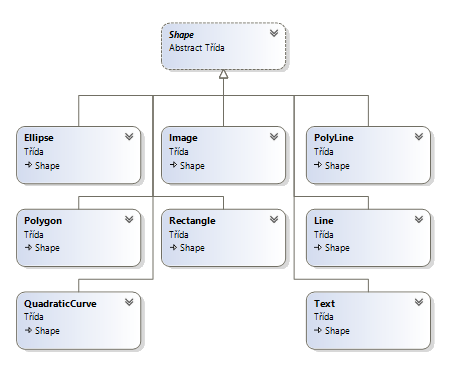
\includegraphics[width=15cm]{img/shape_diag}
\caption{Diagram třídy Shape a jejích potomků}
\end{figure}  

\subsubsection{Editační prvky}
Každý grafický objekt by měl mít k dispozici editační prvky, které zobrazí v momentě, kdy je objekt editován. Editační prvky jsou WPF elementy s naprogramovanými událostmi, které vkládáme při editace do vrchního canvasu, aby je uživatel viděl před objekty a mohl nimi například posouvat.

Například grafický objekt reprezentující čáru, při editace přidává dva maličké kruhy (elipsy). Jelikož tyhle elipsy jsou potřeba při editaci různých grafických objektů, vznikla proto speciálně určená třída.

\paragraph{Třída MovePoint}
Jak jsem již zmínil pro ovládací prvky typu malých elips se kterým jde posouvat, vnikla speciální třída a ta se nazývá \kiinlinecode{csharp}{!}{MovePoint}.

K založení instance je potřeba počáteční bod, instanci grafického objektu, horní canvas a delegát \kiinlinecode{csharp}{!}{void MoveDelegate(Point b)}. Delegát je funkce kterou můžeme ukládat do proměnných  a předávat je jako argumenty funkcí. Náš delegát se zavolá při každé změně pozice a vargumentu dostane bod, kam se přesunu.

Pokud chceme editační prvek zobrazit zavoláme metodu \kiinlinecode{csharp}{!}{Show()}. V opačném případě metodu \kiinlinecode{csharp}{!}{Hide()}

\kiinlinecode{csharp}{!}{MovePoint} automaticky ukládá všechny přesuny do historie.

\paragraph{Třída EditRect}


\subsection{Třída HistoryControl}

Každý soubor má svojí historii všech změn, které při práci v souboru provedeme. O tuto historii se stará třída \kiinlinecode{csharp}{!}{HistoryControl}. Každá třída \kiinlinecode{csharp}{!}{FileControl} si při vytvoření instance, vytvoří svou vlastní instanci třídy \kiinlinecode{csharp}{!}{HistoryControl}.

\kiinlinecode{csharp}{!}{HistoryControl} v sobě uchovává dva zásobníky. První slouží k historii a jsou v něm uloženy akce, které byly provedeny. Do druhého zásobníku se přesouvají akce z prvního, pokud se v historii vracíme zpět. Když půjdeme vpřed, akce z druhého zásobníků se naopak přesune do prvního. Pokud provedeme nějakou změnu, zásobník určený pro kroky vpřed je vyprázdněn.

Jednotlivé akce jsou reprezentovány objekty, které jsou reprezentovány instancí tříd, které implementují rozhraní \kiinlinecode{csharp}{!}{IHistoryNode}.

\subsubsection{Metody třídy}

Třída \kiinlinecode{csharp}{!}{HistoryControl} má následující veřejné metody:

\begin{itemize}
\item \kiinlinecode{csharp}{!}{void Enable()}
\end{itemize}
Při vytvoření instance třídy \kiinlinecode{csharp}{!}{HistoryControl} je historie deaktivována. Zavoláním této metody, spustíme celou funkcionalitu třídy.

\begin{itemize}
\item \kiinlinecode{csharp}{!}{void Add(IHistoryNode node)}
\end{itemize}
Tato metoda slouží k přidáváním akce do historie.

\begin{itemize}
\item \kiinlinecode{csharp}{!}{void Clear()}
\end{itemize}
Smaže celou historii.

\begin{itemize}
\item \kiinlinecode{csharp}{!}{void Back()}
\item \kiinlinecode{csharp}{!}{void Forward()}
\end{itemize}
Pohyb v historii vpřed a vzad, pokud tento přesun není možný, nic se neprovede.

\begin{itemize}
\item \kiinlinecode{csharp}{!}{void SetNotChange()}
\end{itemize}
Nastaví stav, tak že neproběhla žádná změna. Volá si při uložení souboru.

\begin{itemize}
\item \kiinlinecode{csharp}{!}{bool Change()}
\end{itemize}
Testuje, jestli od posledního zavolání \kiinlinecode{csharp}{!}{SetNotChange()} nebo od vytvoření zapnutí historie, se nějak změnila historie. Používá se k testu jestli je potřeba soubor uložit. Aplikace tento test používá k tomu, aby jsme omylem nezavřeli aplikaci bez uložení.

\subsubsection{IHistoryNode}
\kiinlinecode{csharp}{!}{IHistoryNode} je rozhraní, které musí implementovat všechny třídy, které mají implementovat jednotlivé akce v historii.

Každá třída implementující tohle rozhraní, musí implementovat následující dvě metody:

\begin{itemize}
\item \kiinlinecode{csharp}{!}{void Back()}
\end{itemize}
Zde je potřeba naprogramovat co se má stát, pokud chceme tuto akci vrátit zpět.

\begin{itemize}
\item \kiinlinecode{csharp}{!}{void Back()}
\end{itemize}
Opačný přístup, a provede se pokud je akce již minimálně jednou v historii vrácena a má se zase vrátit do původního stavu.

\paragraph{Rozšíření IHistoryNodeSkipped}
Rozhraní \kiinlinecode{csharp}{!}{IHistoryNodeSkipped} je rozšíření rozhraní \kiinlinecode{csharp}{!}{IHistoryNode}. \kiinlinecode{csharp}{!}{HistoryControl} se však k němu chová odlišně.

Pokud metoda \kiinlinecode{csharp}{!}{Add(IHistoryNode node)} třídy \kiinlinecode{csharp}{!}{HistoryControl} dostane instanci třídy implementující rozhraní \kiinlinecode{csharp}{!}{IHistoryNodeSkipped}, tak provede následující kroky:

\begin{itemize}
\item Otestuje, jestli je zásobník určený pro akce zpět prázdný, pokud je prázdný, postupuje klasickým způsobem.
\item Pokud zásobník prázdný není, otestuje jestli akce ležící na vrcholu zásobníku neimplementuje rozhraní \kiinlinecode{csharp}{!}{IHistoryNodeSkipped}. Pokud ho neimplementuje, postupuje klasicky.
\item Vkládaná akce s akci ležící na vrcholu zásobníku jsou otestovány, jestli jsou kompatibilní, pokud ano, akce se spojí a vloží na vrchol zásobníku. V opačném případě se vloží vkládaná akce na vrchol zásobníku.
\end{itemize}

Test jestli jsou dvě akce \kiinlinecode{csharp}{!}{IHistoryNodeSkipped} kompatibilní se provádí metodou \kiinlinecode{csharp}{!}{bool Optimal(IHistoryNodeSkipped node)}, která vrací pravdivostní hodnotu, zda jsou kompatibilní.

Spojení dvou akcí se provádí metoda \kiinlinecode{csharp}{!}{void Skip(IHistoryNodeSkipped node)}, kdy spojení probíhá do akce na které je tato metoda volána.


\begin{figure}
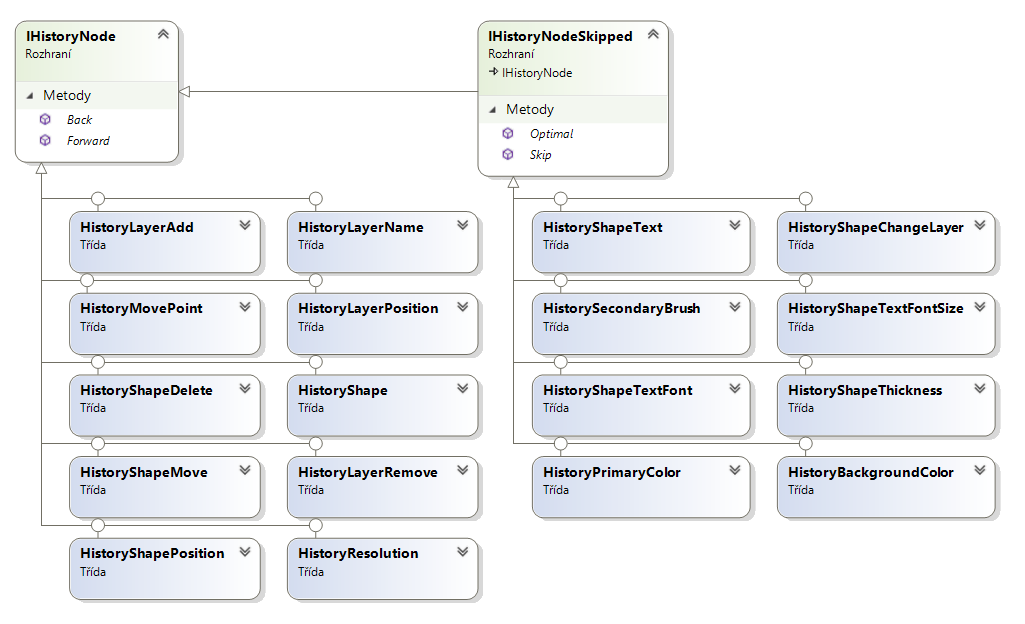
\includegraphics[width=15cm]{img/history_diag}
\caption{Diagram tříd implementující rozhraní IHistoryNode}
\end{figure}  

\section{Funkce}

\subsection{Podporované soubory}

Aplikace podporuje otevírání a ukládání souborů jako rastrovou grafiku ve formátech JPG, PNG a BMP. Při otevření těchto formátů je do plátna načten pouze jeden objekt a tím je celý obrázek. Nelze tak po opětovném otevření upravovat grafické tvary. 

Speciální funkcí této aplikace je ukládání obrázků do formátu HTML. Oproti rastrovým formátům má výhodu v tom, že po otevření jsou načteny do plátna všechny objekty, které je možno dále upravovat. Tento formát reprezentuje obrázek jako vektorovou grafiku. Je možno ho otevřít v jakémkoliv prohlížeči, který podporuje HTML5 Canvas a má zapnutý JavaScript.

\subsubsection{Uložení do souboru ve formátu HTML}

\paragraph{HTML soubor}

Soubor s příponou .html nebo .htm je textový soubor, který obsahuje značkovací jazyk HTML. Jazyk se skládá z tagů (značek), které máme párové a nepárové. Do párových tagů můžeme vkládat další HTML tagy nebo text. Vzniká tak v HTML dokumentu stromová struktura. HTML tagy dále obsahují atributy, které mění vlastnosti tagů.

\begin{kicode}{HTML}{kod:HTML}{Ukázka kódu HTML}
<!DOCTYPE html>
<html>
  <head>
  <meta http-equiv="content-type" content="text/html; charset=utf-8">
  <title>Titulek</title>
  </head>
  <body>
    <h1>Nadpis</h1>
    <p>Text</p>
  </body>
</html>
\end{kicode}

\paragraph{Značka <canvas>}

Formát HTML není určený pro obrázky, ale pro pro webové stránky. Od páté verze HTML podporuje značku <canvas>, která reprezentuje plátno pro kreslení grafiky. Element se umístí do stránky s pevně danou šířkou a výškou. Do plátna pak lze kreslit přes API v JavaScriptu. Pokud změníme jeho rozměry, plátno se vymaže a musíme kreslit znovu.

\begin{kicode}{JavaScript}{kod:JavaScript}{Kreslení obdélníku do canvasu v JavaScriptu}
var c=document.getElementById("myCanvas");
var ctx=c.getContext("2d");
ctx.rect(20,20,150,100);
ctx.stroke();
\end{kicode}

Tahle technologie nám nabízí pomocnou ruku, otázkou je, co uložit do HTML souboru, pokud požadujeme, aby se po otevření souboru ve webovém prohlížeči zobrazil obrázek.

Nabízí se vygenerovat HTML soubor a vložit do něj vygenerovaný program v JavaScriptu, který dokáže obrázek do plátna nakreslit. Tohle řešení by fungovalo, ale mělo by řadu nevýhod. V HTML souboru by bylo spoustu nadbytečného kódu a implementace otevírání HTML souboru, by byla příliš složitá. Nebylo by jednoduché dekódovat program v souboru na grafické objekty. V budoucnu by taky byl problém s kompatibilitou a omezovalo by mě to v případné optimalizaci.

Grafické objekty v aplikaci jsou jen nějaké data uložené v objektech a tak bude jednodušší je tak nechat a zbytečně nepřidávat další balast navíc a to by se přesně stalo, pokud bych se vydal cestou zmíněnou výše. Takže požadujeme tyto objekty uložit do HTML souboru. Protože je HTML soubor textový, musíme tyto objekty reprezentovat pomocí textu. Chceme objekty převést na text a k tomu slouží serializace.

Serializace objektů je proces, který umožňuje objekty programu převést na posloupnost bytů nebo text. Jednoduše umožňuje objekty uložit pro pozdější obnovení.



\paragraph{JSON}
Aplikace používá serializaci do formátu JSON. JSON je datový formát, který dokáže pojmout datové struktury složených z čísel a řetězců. Často se používá k přenosů dat na internetu, hlavně ve ve webových aplikacích, které využívají technologii AJAX. Další obrovskou výhodou je, že pochází z JavaScriptu. Zkratka JSON totiž znamená \uv{JavaScript Object Notation} což je zápis objektů v JavaScriptu a tak nemusíme programovat žádnou deserializaci, ale postačí nám pouze data v tomto formátu do souboru HTML přiložit.


\paragraph{Vykreslení obrázku v prohlížeči}
Posledním krokem k zobrazení obrázku v prohlížeči zbývá vykreslit obrázek z přiložených dat v JSONu. Jak už jsem psal výše použijeme k tomu HTML element <canvas>. Do canvasu se kreslí přes API v JavaScriptu, takže získáme přiložená data musíme dostat do programu v JavaScriptu, který bude z dal obrázek vykreslovat do canvasu. 

Data program získá deserializací JSON řetězce. Jelikož je JSON řetězec ekvivalentní se zápisem objektů v JavaScriptu, postačí nám pouze JSON řetězec šikovně uložit k programu.

Program v JS už jen přečte data a vykreslí všechny grafické objekty ve správném pořadí. Pro menší datovou velikost výsledného HTML souboru je kód programu zminifikován. Minifikace nám z kódu odstraní znaky, které nemají vliv na vykonávání kódu. Což jsou pro příklad bílé znaky (mezery, tabulátory, řádky). Dále nahradí názvy proměnných na co nejkratší názvy. Po minifikaci program dělá to stejné jako před ní, jen je o hodně menší. Minifikace je hojně využívaná na internetu a není se čemu divit, všichni přece chceme, aby se internetové stránky načítaly rychle.

\paragraph{Datová struktura JSONu}
Aby byl program v JavaScriptu schopný nakreslit obrázek z přiložených dat, musí mít data určitou datovou strukturu, je velmi podobná struktuře ve kterém aplikace uchovává data při práci s obrázkem.

Všechno začíná třídou Picture, která uchovává rozlišení obrázku a obsahuje vlastnost layers, ve které je uložen seznam vrstev. Jednotlivé vrstvy jsou reprezentovány třídou Layer, která v sobě uchovává barvu pozadí, jméno vrstvy a jestli je vrstva viditelná, jestli se má vykreslit. Mohli by jsme říct, že je zbytečné přikládat vrstvu, která se stejně nenakreslí, ale jelikož jde HTML soubor v aplikaci znovu otevřít a plnohodnotně editovat je dobré ji tam nechat, kdyby s ní ještě chtěl v budoucnu někdo pracovat. To nejdůležitější co třída Layer obsahuje je seznam grafických objektů  umístěný ve vlastnosti shapes.

Grafické objekty jsou reprezentovány třídou Shape. Různé druhy grafických objektů mají hodně odlišné vlastnosti a proto by nebylo moudré všechno ukládat, použijeme tedy dědičnost. Potomky třídy Shape jsou třídy reprezentující jednotlivé druhy grafických objektů, které v sobě uchovávají barvy výplně a okraje, body ze kterých jsou složeny nebo jiné.

Protože serializací objektů do formátu JSON, přijdeme o informaci o informaci z jaké třídy pochází, jelikož JSON formát tyto informace neuchovává. Řešení je jednoduché, stačí přidat všem třídám reprezentují grafické objekty vlastnost type, kde každý druh bude mít unikátní hodnotu. V našem případě je vlastnost type typu řetězec a obsahuje vždy název své třídy. Díky tomu dokáže program jednoduchým způsobem rozpoznat o jaký druh grafického objektu se jedná a podle toho může očekávat vlastnosti.

Zvláštním případem grafického objektu je obrázek, který reprezentuje třída Image a je to obrázek v rastrové grafice. Umožní nám tak ukládat do HTML i rastrovou grafiku. Obrázek je uložen pomocí kódování base64. Base64 je způsob kódování, který kóduje binární data do znaků ASCII a tak lze tímto způsobem uložit obrázek pomocí řetězce. Celou strukturu zobrazuje diagram na obrázku \ref{fig:json_diag}.

\paragraph{Struktura uloženého souboru}
Máme všechny součásti pro uložení dat do souboru. Aplikace soubory HTML ukládá s následující strukturou (zdrojový kód \ref{kod:HTMLst}).

\begin{kicode}{HTML}{kod:HTMLst}{Struktura HTML souboru}
<!DOCTYPE HTML>
<html>
  <head>
    <meta http-equiv="content-type" content="text/html; charset = utf-8">
  </head>
  <body>
  <canvas width="500" height="400" style="border: 1px solid black;" id="MyPaint"></canvas>
  <script>
    var ctx = document.getElementById("MyPaint").getContext("2d");
    var json = *JSON_RETEZEC*;
    *PROGRAM*
    draw(0, -1);
  </script>
  </body>
</html>
\end{kicode}


\begin{figure}
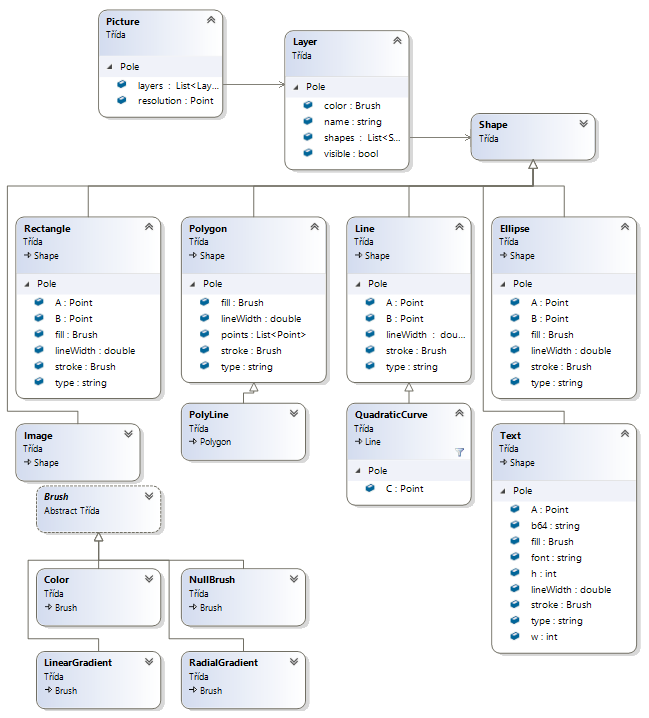
\includegraphics[width=15cm]{img/json_diag}
\caption{Diagram datové struktury pro uložení obrázku do JSONu}
\label{fig:json_diag}
\end{figure} 


\subsubsection{Otevření souboru ve formátu HTML}
Aplikace umožňuje otevřený HTML soubory plnohodnotně editovat. V souboru jsou zachovány všechny vrstvy a grafické objekty, tak jak byly uloženy. To je díky tomu, že v JSONu jsou uloženy všechny informace a i informace, který nemají vliv na grafickou podobu obrázku, což jsou například jména vrstev. Stejný přístup využívá aplikace Adobe Photoshop, kde můžeme obrázky ukládat do formátu PSD, který též zachová všechny elementy.

Aplikace najde v HTML JSON řetězec a následně deserializuje řetězec. Z dat získaných z deserializovaného řetězce sestaví data pro soubor reprezentovaný v aplikaci a otevře ho v nové záložce.

\subsubsection{Uložení do formátů rastrové grafiky}
Aplikace umožňuje uložit obrázky do rastrové (bitmapové) grafiky. Rastrová grafika je způsob ukládání obrázků. Obrázek tímto způsobem je uložen jako barevné body (pixelů, kde každý bod má svojí barvu. Barva pixelů je vyjádřena ve vybraném barevném modelu, v modelu kde můžeme z posloupnosti čísel získat barvu, například model RGB, kde ze třech čísel reprezentující 3 barvy (konkrétně červená, zelená a modrá) dostaneme výslednou barvou jejich smícháním. Existuje i rozšíření modelu RGB, což je model RGBa, kde je navíc ještě čtvrtá složka (alfa kanál), která určuje průhlednost barvy.

Implementace uložení do rastrové grafiky v Aplikaci je poměrně jednoduchá. Knihovna WPF umožňuje zachytit obrázek jakéhokoliv elementu, který se v GUI aplikace nachází. Aplikace ale nezachycuje přímo plátno ve kterém probíhá práce na obrázku, ale pro urychlení vytvoří nové vlákno. V novém vlákně aplikace vytvoří nový element plátna a do něj přidá všechny objekty, které mají být v obrázku vidět. Následně vyfotí plátno a výsledný obrázek už se pouze zakóduje do příslušného formátu a soubor s obrázkem uloží na disk.


\section{Uživatelské rozhraní}

Následující kapitola popisuje rozložení prvků v uživatelském rozhraní a jejich funkce.

\subsection{Horní panel}
Horní panel aplikace slouží pro výběr nástroje pro práci. Funguje jako přepínač, současně lze zvolit pouze jeden nástroj. Následně uvedu jednotlivé nástroje.

\begin{itemize}
\item Nástroj pro výběr - slouží pro výběr části obrázku, který lze následně klávesovou zkratkou Ctrl+C zkopírovat do schránky a vložit výřez do jiného programu, nebo jej naklonovat.
\item Nástroj pro výběr grafických objektů - slouží pro označení objektu, který chceme editovat.
\item Úsečka - pro kreslení obyčejné úsečky mezi dvěma body.
\item Polyline - Křivka vytvořená spojením n bodů.
\item Elipsa
\item Obdélník
\item Polygon
\item Kvadratická křivka
\item Text
\item Zpět
\item Vpřed
\item Nástroje pro změnu vlastnosti písma (zobrazí se pouze při editaci textu)
\end{itemize}
\newpage
\begin{figure}
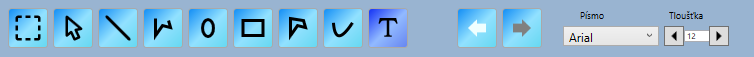
\includegraphics[width=16cm]{img/toppanel}
\caption{Horní panel}
\end{figure}


\subsection{Levý panel}

Horní část levého panelu slouží pro nastavení vlastností grafický objektů. Mezi hlavní vlastnosti patří barvy. V aplikaci můžeme každému objektu nastavit 2 různé barvy: primární a sekundární. Primární slouží u objektů jako barva okraje a sekundární jako barva výplně. Každý objekt však nemá výplň. Například taková úsečka nebo kvadratická křivka výplň nemá a tak na nastavení této vlastnosti nebude reagovat. 

Dále tu máme třetí barvu, která slouží pro nastavení pozadí aktuální vrstvy.

Nastavování těchto těch barev se provádí s pomocí přepínače. Zvolíme jednu z nich a následně jim nastavíme požadovanou barvu. Výběr je možno provést pomocí základních nadefinovaných barev umístěných níže. Pro pokročilejší výběr máme k dispozici paletu barev. Kromě jedné barvy lze nastavit i průhledná nebo přechod více barev.

Na spodní části levého panelu nalezneme správu vrstev. Zde můžeme vrstvy přidávat a nebo mezi nimi přepínat a tak měnit aktivní vrstvu do které aktuálně chceme kreslit. Dále můžeme jednotlivé vrstvy mazat nebo měnit jejich jména či pořadí.

\begin{figure}
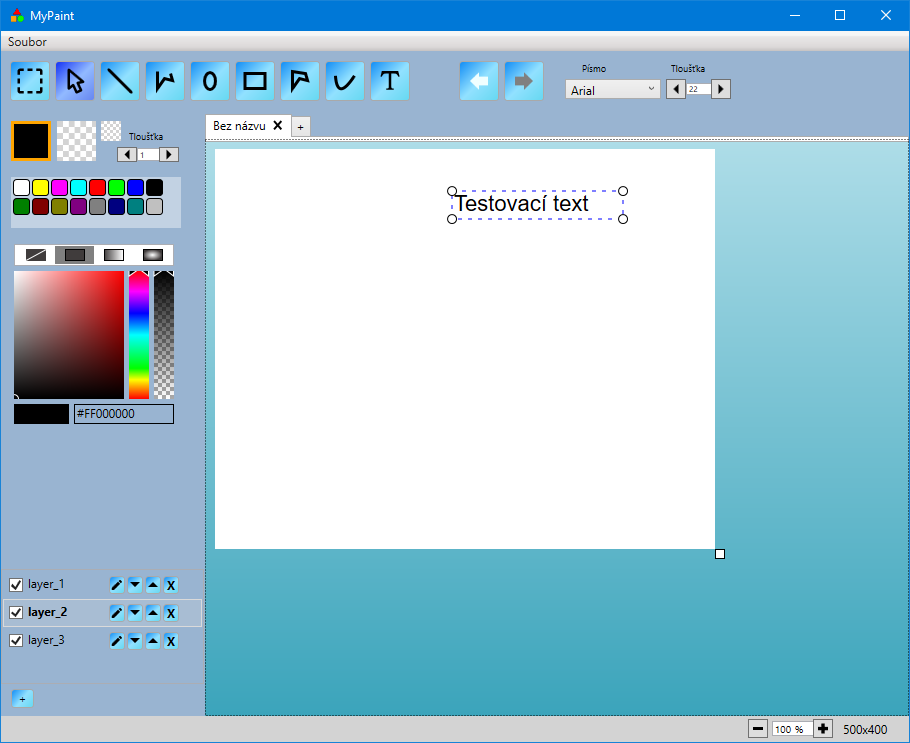
\includegraphics[width=15cm]{img/program}
\caption{Aplikace}
\end{figure}  

\subsection{Kreslící plátno}

Ve středu aplikace se nachází kreslící plátno. Zde můžeme vytvářet a následně upravovat grafické objekty. V pravém dolním rohu kreslícího plátna je umístěn bod pro změnu velkosti plátna. Nad plátnem jsou záložky pro otevřené soubory, program totiž umožňuje upravovat více obrázků najednou.




%% Závěry práce. V jazyce práce a anglicky. Text pro jiný než
%% nastavený jazyk práce (nepovinným parametrem language makra
%% \documentclass, výchozí český) se zadává použitím makra s uvedením
%% jazyka jako nepovinného parametru.
\begin{kiconclusions}
Závěr práce v \uv{českém} jazyce.
\end{kiconclusions}

\begin{kiconclusions}[english]
Thesis conclusions in \uv{English}.
\end{kiconclusions}

%% Přílohy obsahu textu práce, za makrem \appendix.
\appendix

\section{První příloha}
Text první přílohy

\section{Druhá příloha}
Text druhé přílohy

%% Obsah přiloženého CD/DVD. Poslední příloha. Upravte podle vlastní
%% práce!
\section{Obsah přiloženého CD/DVD} \label{sec:ObsahCD}

Na samotném konci textu práce je uveden stručný popis obsahu
přiloženého CD/DVD, tj.~jeho závazné adresářové struktury, důležitých
souborů apod.

\begin{description}

\item[\texttt{bin/}] \hfill \\
  Instalátor \textsc{Instalator} programu, popř.~program
  \textsc{Program}, spustitelné přímo z~CD/DVD. / Kompletní adresářová
  struktura webové aplikace \textsc{Webovka} (v~ZIP archivu) pro
  zkopírování na webový server. Adresář obsahuje i~všechny runtime
  knihovny a~další soubory potřebné pro bezproblémový běh instalátoru
  a~programu z~CD/DVD / pro bezproblémový provoz webové aplikace na
  webovém serveru.

\item[\texttt{doc/}] \hfill \\
  Text práce ve formátu PDF, vytvořený s~použitím závazného stylu KI
  PřF UP v~Olomouci pro závěrečné práce, včetně všech příloh,
  a~všechny soubory potřebné pro bezproblémové vygenerování PDF
  dokumentu textu (v~ZIP archivu), tj.~zdrojový text textu, vložené
  obrázky, apod.

\item[\texttt{src/}] \hfill \\
  Kompletní zdrojové texty programu \textsc{Program} / webové aplikace
  \textsc{Webovka} se všemi potřebnými (příp.~převzatými) zdrojovými
  texty, knihovnami a~dalšími soubory potřebnými pro bezproblémové
  vytvoření spustitelných verzí programu / adresářové struktury pro
  zkopírování na webový server.

\item[\texttt{readme.txt}] \hfill \\
  Instrukce pro instalaci a~spuštění programu \textsc{Program}, včetně
  všech požadavků pro jeho bezproblémový provoz. / Instrukce pro
  nasazení webové aplikace \textsc{Webovka} na webový server, včetně
  všech požadavků pro její bezproblémový provoz, a~webová adresa, na
  které je aplikace nasazena pro účel testování při tvorbě posudků
  práce a~pro účel obhajoby práce.

\end{description}

Navíc CD/DVD obsahuje:

\begin{description}

\item[\texttt{data/}] \hfill \\
  Ukázková a~testovací data použitá v~práci a~pro potřeby testování
  práce při tvorbě posudků a~obhajoby práce.

\item[\texttt{install/}] \hfill \\
  Instalátory aplikací, runtime knihoven a~jiných souborů potřebných
  pro provoz programu \textsc{Program} / webové aplikace
  \textsc{Webovka}, které nejsou standardní součástí operačního
  systému určeného pro běh programu / provoz webové aplikace.

\item[\texttt{literature/}] \hfill \\
  Vybrané položky bibliografie, příp.~jiná užitečná literatura
  vztahující se k~práci.

\end{description}

U~veškerých cizích převzatých materiálů obsažených na CD/DVD jejich
zahrnutí dovolují podmínky pro jejich šíření nebo přiložený souhlas
držitele copyrightu. Pro všechny použité (a~citované) materiály,
u~kterých toto není splněno a~nejsou tak obsaženy na CD/DVD, je uveden
jejich zdroj (např.~webová adresa) v~bibliografii nebo textu práce
nebo v souboru \texttt{readme.txt}.

%% -------------------------------------------------------------------

%% Sazba volitelného seznamu zkratek, za přílohami.
\printglossary

%% Sazba povinné bibliografie, za přílohami (případně i za seznamem
%% zkratek). Při použití BibLaTeXu použijte makro
%% \printbibliography. jinak prostředí thebibliography. Ne obojí!

%% Sazba i v textu necitovaných zdrojů, při použití
%% BibLaTeXu. Volitelné.
\nocite{*}
%% Vlastní sazba bibliografie při použití BibLaTeXu.
\printbibliography

%% Bibliografie, včetně sazby, při nepoužití BibLaTeXu.
% \begin{thebibliography}{9}
%\bibitem{kniha2} \uppercase{Hawke}, Paul. NanoHttpd: Light-weight HTTP server designed for embedding in other applications. GitHub [online]. 2014-05-12. [cit. 2014-12-06]. Dostupné z: \url{https://github.com/NanoHttpd/nanohttpd}
%
%\bibitem{jeske13} \uppercase{Jeske}, David; \uppercase{Novák}, Josef. Simple HTTP Server in \csharp: Threaded synchronous HTTP Server abstract class, to respond to HTTP requests. CodeProject: For those who code [online]. 2014-05-24. [cit. 2014-12-06]. Dostupné z: \url{http://www.codeproject.com/Articles/137979/Simple-HTTP-Server-in-C}
%
%\bibitem{uzis2012} \uppercase{ÚSTAV ZDRAVOTNICKÝCH INFORMACÍ A STATISTIKY ČR}. Lékaři, zubní lékaři a farmaceuti 2012 [online]. Praha 2, Palackého náměstí 4: Ústav zdravotnických informací a statistiky ČR, 2012 [cit. 2014-12-06]. ISBN 978-80-7472-089-5. Dostupné z: \url{http://www.uzis.cz/publikace/lekari-zubni-lekari-farmaceuti-2012}
% \end{thebibliography}

%% Sazba volitelného rejstříku, za bibliografií.
\printindex

\end{document}
